% Generated from the longer deck; rebuild with scripts/build_backups.py.


\section{Appendix index}

\renewcommand{\backupcode}{Index}

\begin{frame}[more-space,label=backup-index]{Appendix\enspace|\enspace Topic index}

\par\medskip

{\renewcommand{\arraystretch}{1.8}

\begin{tabular}{@{}p{0.44\textwidth}p{0.52\textwidth}@{}}

\toprule\textbf{Topic} & \textbf{Appendix codes}\\\midrule

\textbf{A. Data and preprocessing} & \hyperlink{backup-A1}{\color{rwth-blue-100}\textbf{A1}}\quad \hyperlink{backup-A2}{\color{rwth-blue-100}\textbf{A2}}\quad \hyperlink{backup-A3}{\color{rwth-blue-100}\textbf{A3}}\quad \hyperlink{backup-A4}{\color{rwth-blue-100}\textbf{A4}}\quad \hyperlink{backup-A5}{\color{rwth-blue-100}\textbf{A5}}\quad \hyperlink{backup-A6}{\color{rwth-blue-100}\textbf{A6}}\quad \hyperlink{backup-A7}{\color{rwth-blue-100}\textbf{A7}}\\

\textbf{B. PCE and input reference} & \hyperlink{backup-B1}{\color{rwth-blue-100}\textbf{B1}}\quad \hyperlink{backup-B2}{\color{rwth-blue-100}\textbf{B2}}\quad \hyperlink{backup-B3}{\color{rwth-blue-100}\textbf{B3}}\quad \hyperlink{backup-B4}{\color{rwth-blue-100}\textbf{B4}}\\

\textbf{C. PI-PCE and comparison} & \hyperlink{backup-C1}{\color{rwth-blue-100}\textbf{C1}}\quad \hyperlink{backup-C2}{\color{rwth-blue-100}\textbf{C2}}\quad \hyperlink{backup-C3}{\color{rwth-blue-100}\textbf{C3}}\quad \hyperlink{backup-C4}{\color{rwth-blue-100}\textbf{C4}}\quad \hyperlink{backup-C5}{\color{rwth-blue-100}\textbf{C5}}\quad \hyperlink{backup-C6}{\color{rwth-blue-100}\textbf{C6}}\quad \hyperlink{backup-C7}{\color{rwth-blue-100}\textbf{C7}}\quad \hyperlink{backup-C8}{\color{rwth-blue-100}\textbf{C8}}\\

\textbf{D. UQ and sensitivity} & \hyperlink{backup-D1}{\color{rwth-blue-100}\textbf{D1}}\quad \hyperlink{backup-D2}{\color{rwth-blue-100}\textbf{D2}}\\

\textbf{E. Digital twin and operating choices} & \hyperlink{backup-E1}{\color{rwth-blue-100}\textbf{E1}}\quad \hyperlink{backup-E2}{\color{rwth-blue-100}\textbf{E2}}\quad \hyperlink{backup-E3}{\color{rwth-blue-100}\textbf{E3}}\quad \hyperlink{backup-E4}{\color{rwth-blue-100}\textbf{E4}}\\

\textbf{F. Outlook} & \hyperlink{backup-F1}{\color{rwth-blue-100}\textbf{F1}}\\

\bottomrule\end{tabular}}

\medskip

\end{frame}

\section{Appendix A: Data and preprocessing}

\renewcommand{\backupcode}{A1}

\begin{frame}[more-space,label=backup-A1]{A1\enspace|\enspace Operating cases and measured ranges}
  \begin{columns}[T,onlytextwidth]
    \column{0.47\textwidth}
      \dataheading{Measured variables}
      {\footnotesize
      \renewcommand{\arraystretch}{1.25}
      \setlength{\tabcolsep}{4pt}
      \begin{tabular*}{\linewidth}{@{\extracolsep{\fill}}lr@{}}
        \toprule
        \textbf{Model input} & \textbf{Observed range}\\
        \midrule
        Total CPU power & 329--2,312 W\\
        Inlet air temperature & 23.4--46.4\,${}^\circ$C\\
        Raw fan signal (unverified unit) & 0.117--0.766\\
        \midrule
        \textbf{Response} & \\
        Maximum CPU temperature & 36--95\,${}^\circ$C\\
        \bottomrule
      \end{tabular*}
      \smallskip      }

    \column{0.50\textwidth}
      \dataheading{Five operating regimes}
      {\footnotesize
      \renewcommand{\arraystretch}{1.12}
      \setlength{\tabcolsep}{4pt}
      \begin{tabular*}{\linewidth}{@{\extracolsep{\fill}}lr@{}}
        \toprule
        \textbf{Case} & \textbf{Inlet} $[{}^\circ\mathrm{C}]$\\
        \midrule
        \casekey{caseone}{1}   & 25\\
        \casekey{casetwo}{2}   & 35\\
        \casekey{casethree}{3} & 45\\
        \casekey{casefour}{4}  & 45\\
        \casekey{casefive}{5}  & 45\\
        \bottomrule
      \end{tabular*}
      \smallskip
      CPU stress tests for every case: \textbf{100 / 75 / 50 / 25\,\% / idle}      }
  \end{columns}
  \par\vspace{4mm}
  % Center the load panel from the preprocessing slide beneath both tables.
  \noindent\makebox[\textwidth][c]{%
    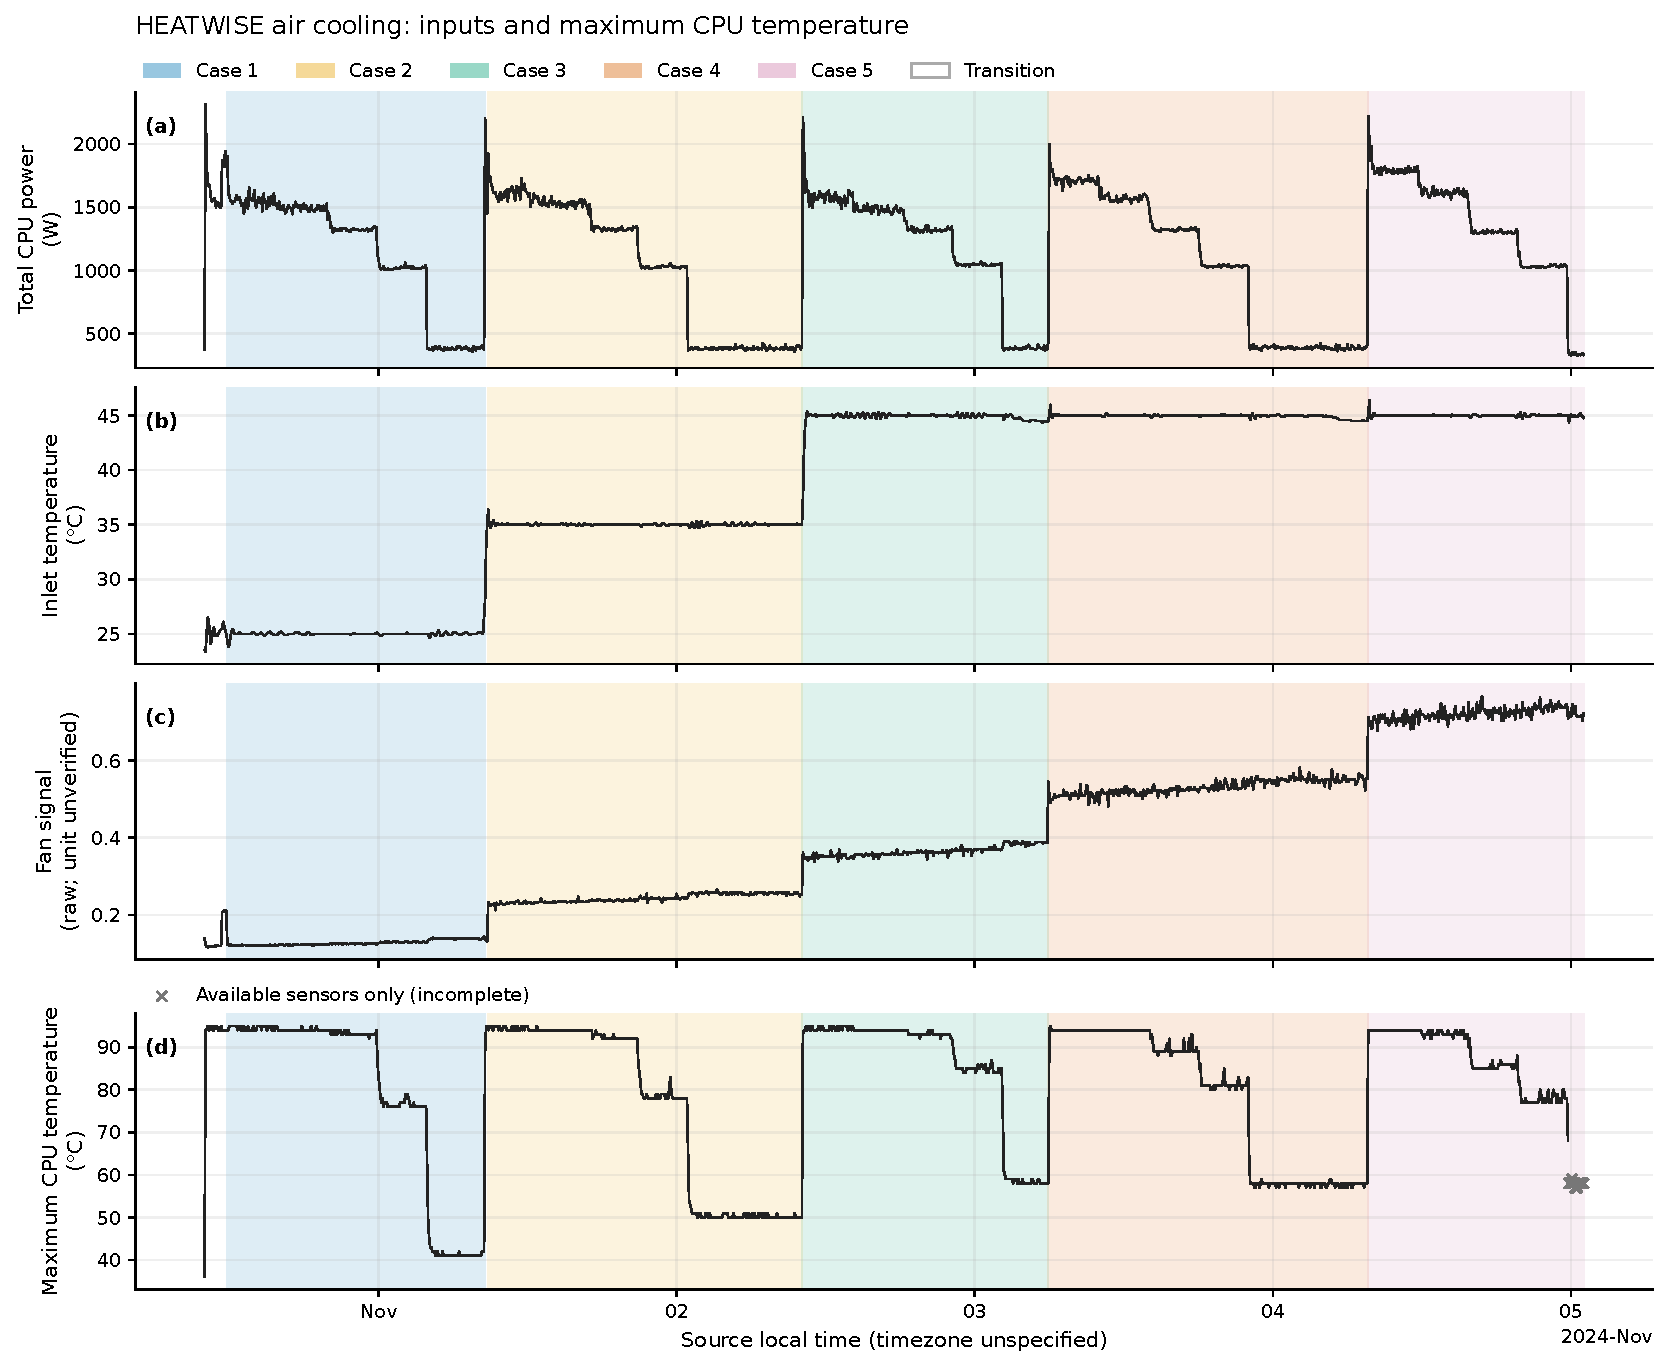
\includegraphics[width=0.65\textwidth,trim=0bp 478bp 0bp 22bp,clip]
      {../../results/audit/figures/inputs_and_max_temperature_timeseries.pdf}%
  }
  \par\vspace{1mm}
  \noindent\makebox[\textwidth][c]{\footnotesize Total CPU power over elapsed time}
\end{frame}

\renewcommand{\backupcode}{A2}

\begin{frame}[more-space,label=backup-A2]{A2\enspace|\enspace Coverage, fan units and throttling}
  \begin{columns}[T,onlytextwidth]
    \column{0.51\textwidth}
      \dataheading{Observed inlet / fan combinations}
      \centering
      % Panel (a) of the existing vector figure; other panels and the shared
      % legend are clipped only at display time. Source PDF stays unchanged.
      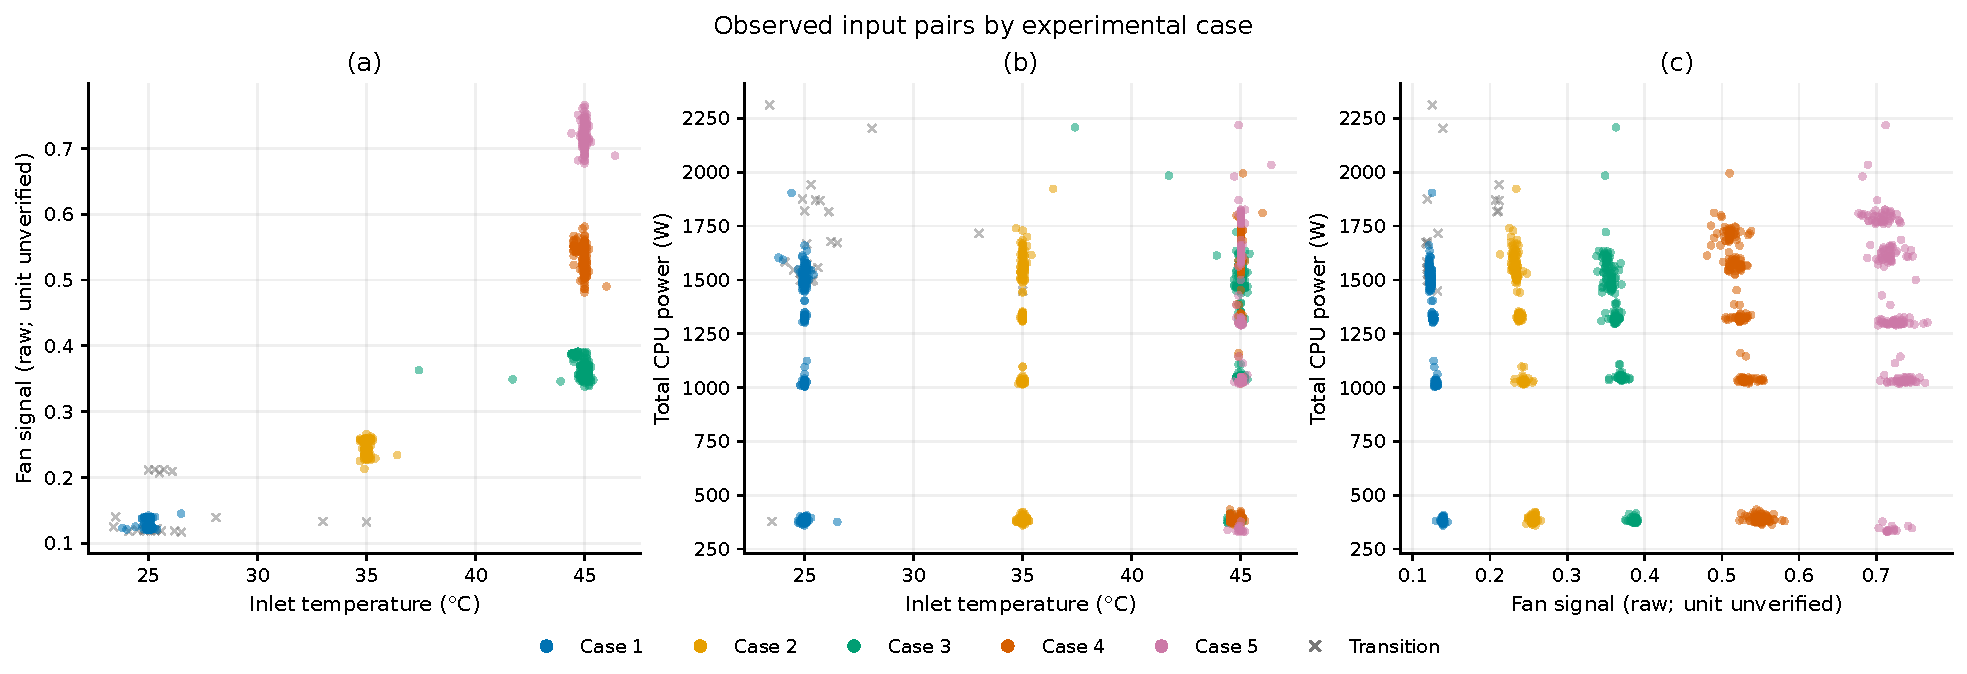
\includegraphics[width=\linewidth,height=49mm,keepaspectratio,
        trim=0bp 24bp 634bp 40bp,clip]
        {../../results/audit/figures/pairwise_input_scatter.pdf}
      \par\smallskip
      {\footnotesize
        \casekey{caseone}{1}\quad\casekey{casetwo}{2}\quad
        \casekey{casethree}{3}\quad\casekey{casefour}{4}\quad
        \casekey{casefive}{5}\quad{\color{black!50}$\times$}\,transition
      }

    \column{0.46\textwidth}
      \begin{beamercolorbox}[sep=2mm,wd=\linewidth]{data warning}
        \dataheading{1. Sparsity}
        {\large\color{rwth-blue-100}\bfseries 31 / 125}\;occupied grid cells\par
        \smallskip
        \begin{itemize}
          \setlength{\itemsep}{1pt}
          \vspace{-1.5mm}
          \item Five trajectories; no full factorial design or LHS.
          \item \textbf{Untested:} high fan signals between $25\,{}^\circ$C and $45\,{}^\circ$C.
        \end{itemize}
        \vspace{-1.5mm}
      \end{beamercolorbox}

      \medskip
      \begin{beamercolorbox}[sep=2mm,wd=\linewidth]{data warning}
        \dataheading{2. Unverified unit of fan signal}
        \begin{itemize}
          \vspace{-1.5mm}
          \item \textbf{Needed:} confirmation from data owners.
        \end{itemize}
        \vspace{-1.5mm}
      \end{beamercolorbox}

      \medskip
      \begin{beamercolorbox}[sep=2mm,wd=\linewidth]{data warning}
        \dataheading{3. Suspected CPU throttling}
        \footnotesize
        \begin{itemize}
          \setlength{\itemsep}{1pt}
          \vspace{-1.5mm}
          \item \textbf{6 targets \boldmath$\geq$\,93.5\,\textdegree C}; all are kept.
          \item A temperature flag, not confirmation from frequency data.
          \item Throttling can mask the power--temperature trend.
        \end{itemize}
        \vspace{-1.5mm}
      \end{beamercolorbox}
      \end{columns}
\end{frame}

\renewcommand{\backupcode}{A3}

\begin{frame}[more-space,label=backup-A3]{A3\enspace|\enspace Input dependence}
  \begin{columns}[T,onlytextwidth]
    \column{0.66\textwidth}
      \dataheading{Observed correlations between the model inputs}
      % Use the existing vector figure in place; trim its redundant top title.
      % Both correlation matrices, tick labels, and the color scale are retained.
      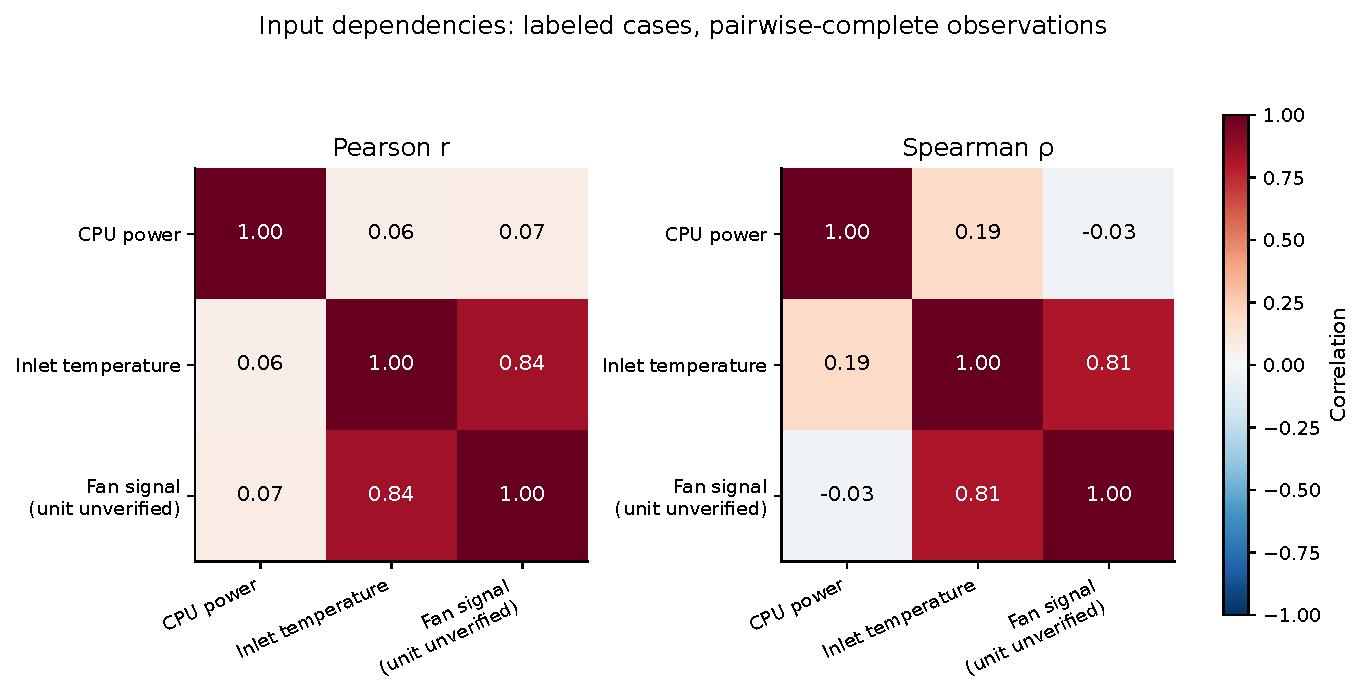
\includegraphics[width=\linewidth,trim=0bp 0bp 0bp 35bp,clip]
        {../../results/audit/figures/input_correlation_matrix.pdf}
      \par\smallskip

    \column{0.31\textwidth}
      \begin{beamercolorbox}[sep=2mm,wd=\linewidth]{data warning}
        \dataheading{4. Input Dependence}
        \textbf{Fan signal - Inlet temperature}\par
        \smallskip
        {\large\color{rwth-blue-100}\bfseries $r=0.84$\quad $\rho=0.81$}\par
      \end{beamercolorbox}

      \medskip
      \dataheading{Our decision:}
      \footnotesize
      \begin{itemize}
        \item For PCE, we decided to treat inputs as \textbf{independent}, with \textbf{equal weight across each range}.
        \item So, Sobol indices show which inputs matter \textbf{under these assumptions}.
        \item Real inputs vary together.
        \item Input dependence will be addressed later.
      \end{itemize}
  \end{columns}
\end{frame}

\renewcommand{\backupcode}{A4}

\begin{frame}[c,more-space,label=backup-A4]{A4\enspace|\enspace Why approximately steady targets?}
  \begin{tikzpicture}[remember picture,overlay]
    \node[anchor=center,inner sep=0pt] at (current page.center) {%
      \begin{minipage}{\textwidth}
  \begin{beamercolorbox}[sep=1.5mm,wd=\textwidth]{data panel}
    \dataheading{Our static PCE predicts approximately steady temperatures}
    \small
    This model has no time or state input: it does not predict transients.\par
    \smallskip
    $\Longrightarrow$ \textbf{We need to select settled operating periods before fitting.}
  \end{beamercolorbox}
      \end{minipage}%
    };
  \end{tikzpicture}
\end{frame}

\renewcommand{\backupcode}{A5}

\begin{frame}[more-space,label=backup-A5]{A5\enspace|\enspace Full preprocessing checklist}
  \begin{columns}[T,onlytextwidth]
    \column{0.56\textwidth}
      \dataheading{Load steps and thermal response}
      % Display panels (a) and (d) from the same existing time-series PDF.
      % The shared case colors and time axis are retained; no data are altered.
      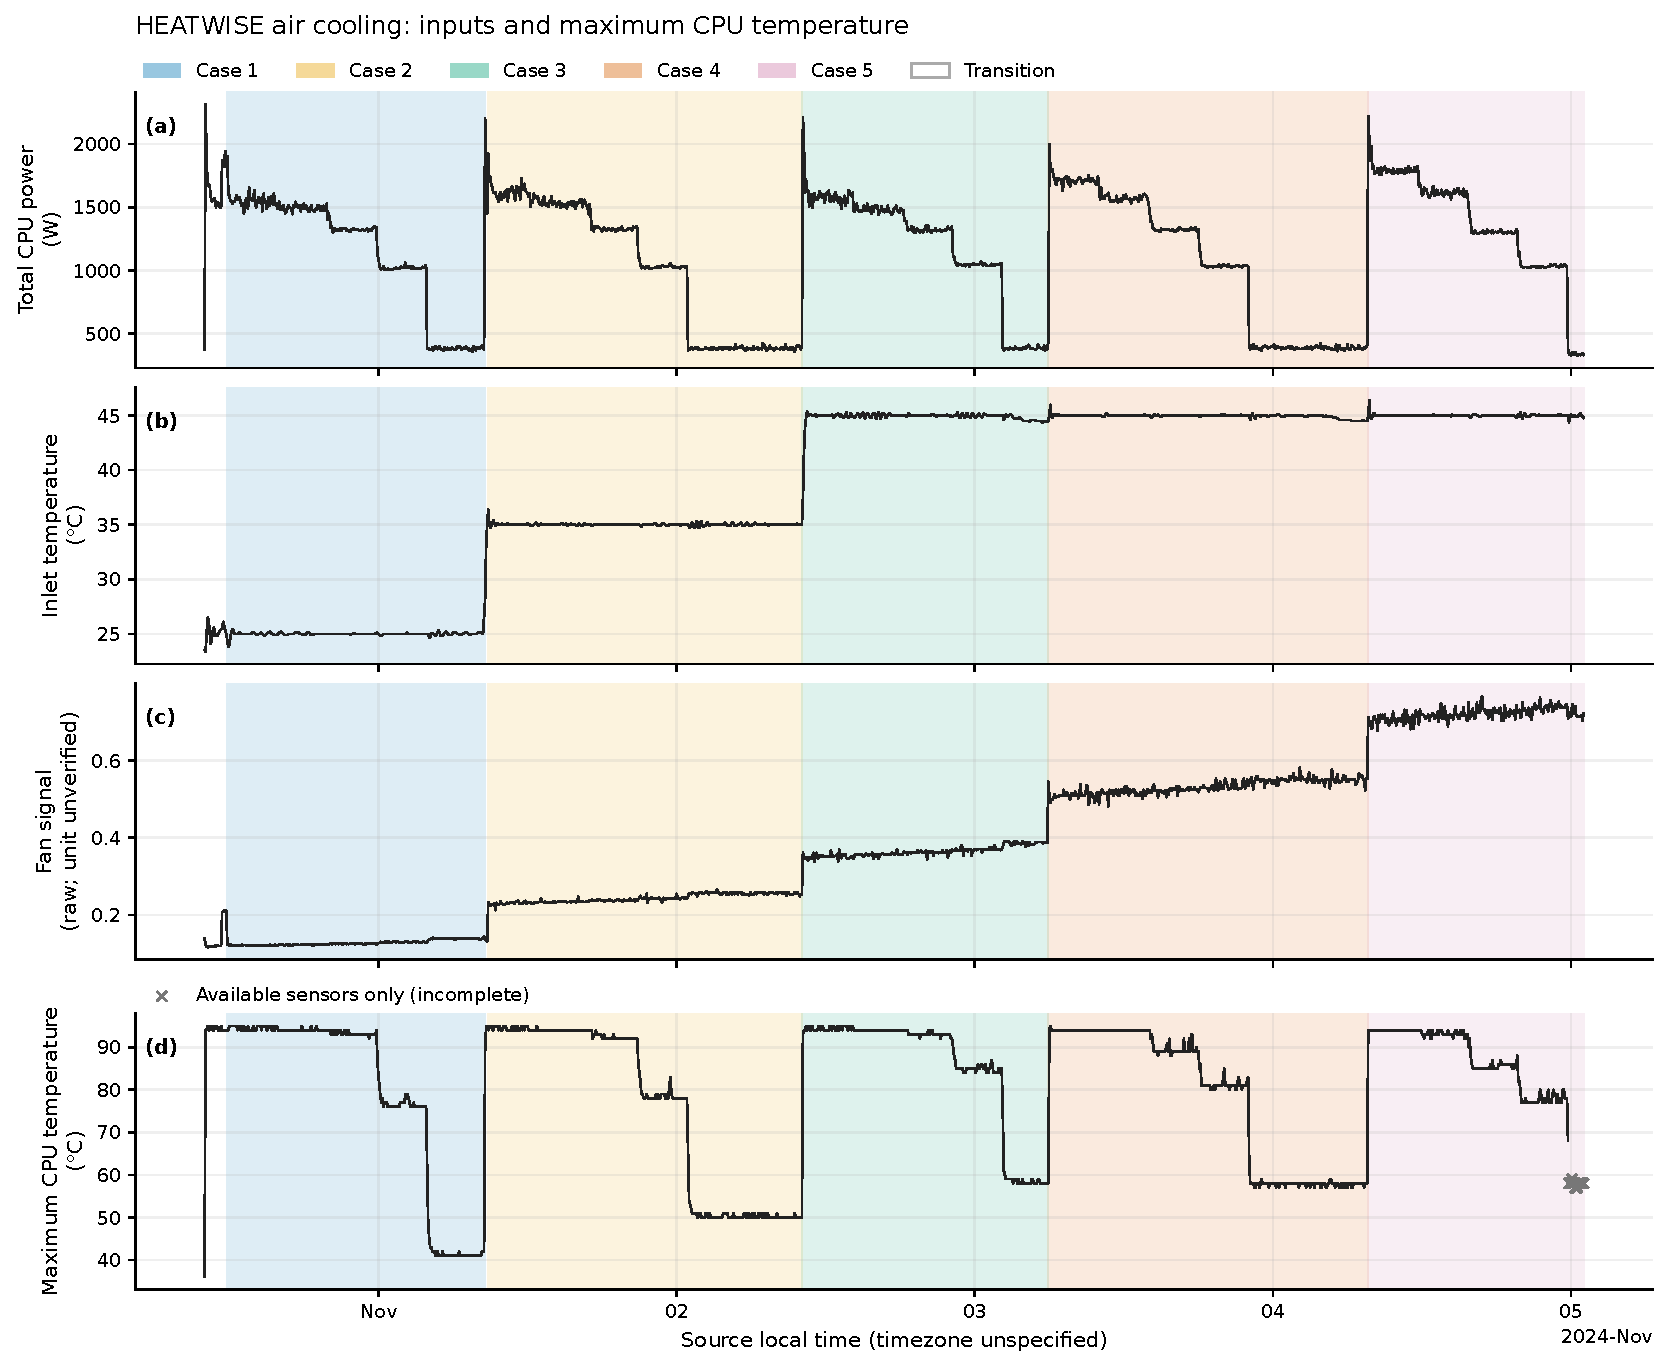
\includegraphics[width=\linewidth,trim=0bp 478bp 0bp 22bp,clip]
        {../../results/audit/figures/inputs_and_max_temperature_timeseries.pdf}
      \par\vspace{1mm}
      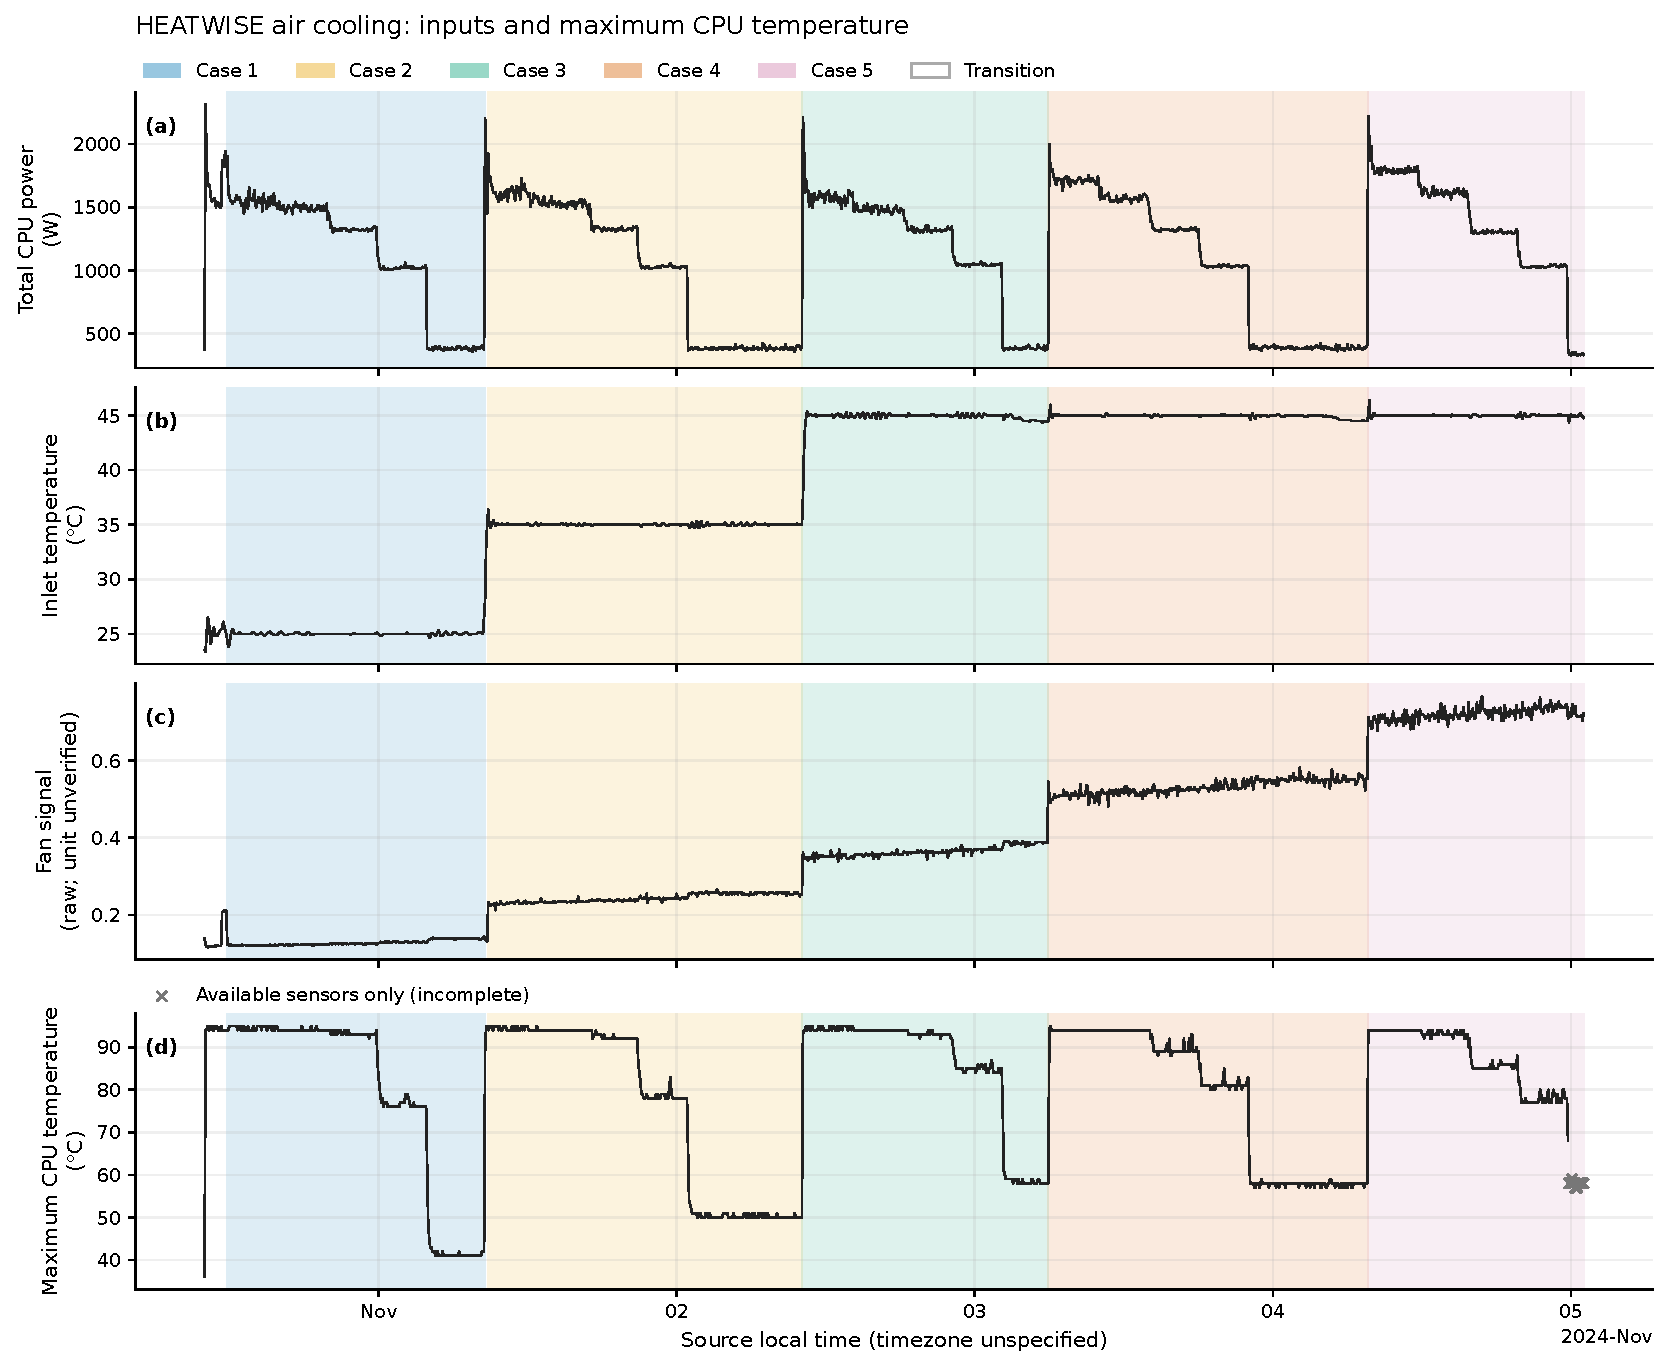
\includegraphics[width=\linewidth,trim=0bp 0bp 0bp 472bp,clip]
        {../../results/audit/figures/inputs_and_max_temperature_timeseries.pdf}
      \par\smallskip
      {\footnotesize Temperatures need time to settle after each load change.}

    \column{0.41\textwidth}
      \begin{beamercolorbox}[sep=2mm,wd=\linewidth]{data panel}
        \dataheading{Approximately steady: selection criteria}
        \small
        \begin{enumerate}
          \item Use \textbf{cases 1--5}; exclude transitions.
          \item Require \textbf{all 18 CPU readings}.
          \item Split periods when input levels change.
          \item Discard the first \textbf{20 minutes}.
          \item Keep at least \textbf{30 continuous minutes}: nearly constant inputs, little temperature fluctuation or drift.
          \item Keep the \textbf{longest passing interval} per period.
        \end{enumerate}
      \end{beamercolorbox}
  \end{columns}
  \medskip
  \begin{beamercolorbox}[sep=1.5mm,wd=\textwidth]{data panel}
    \small
    \textbf{One accepted interval $\rightarrow$ one processed row:}
    average the inputs; target = largest of the 18 CPU temperature averages.
  \end{beamercolorbox}
\end{frame}

\renewcommand{\backupcode}{A6}

\begin{frame}[more-space,label=backup-A6]{A6\enspace|\enspace Selection results and the 19 observations}
  \begin{columns}[T,onlytextwidth]
    \column{0.56\textwidth}
      \dataheading{Selected approximately steady intervals}
      \centering
      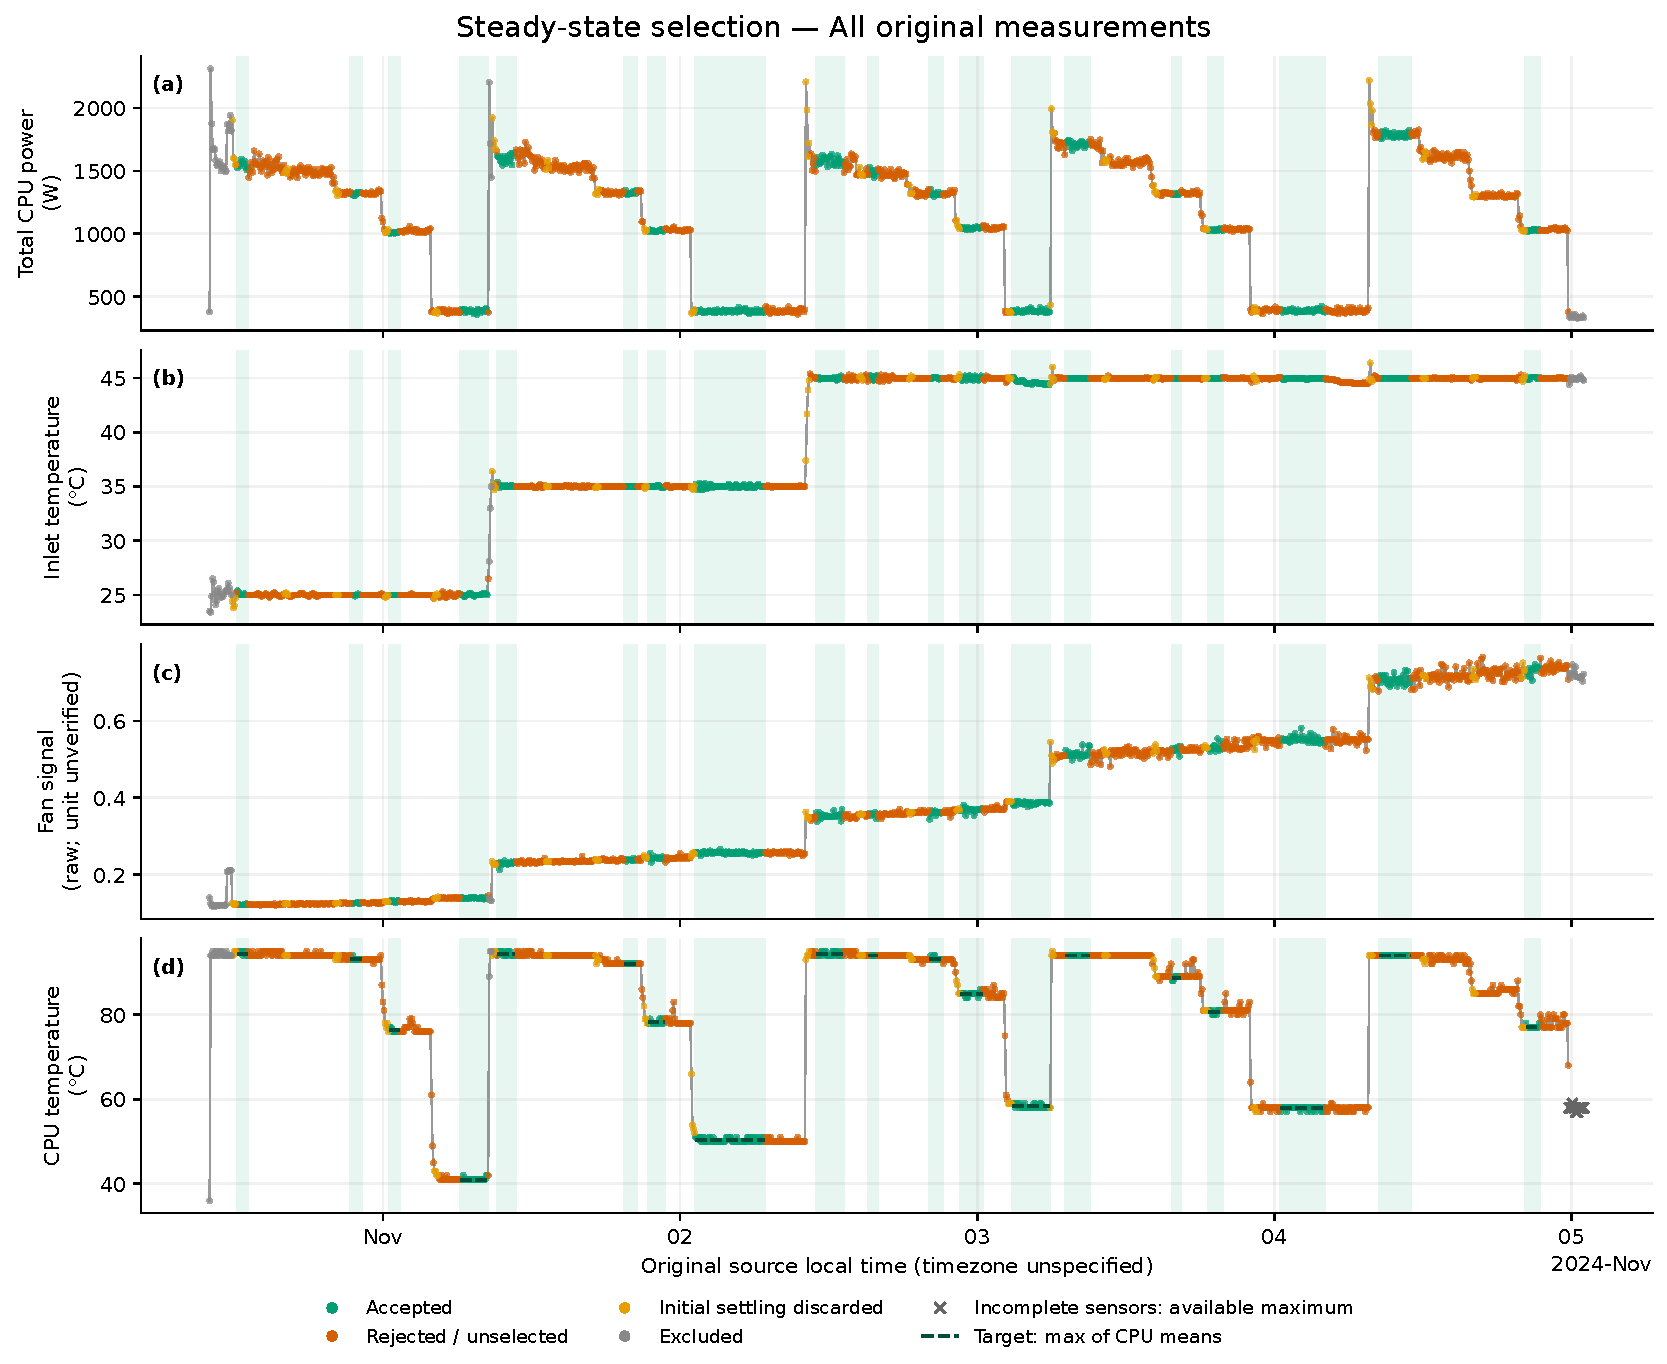
\includegraphics[width=\linewidth,height=50mm,keepaspectratio]
        {../../results/preprocessing/figures/selection_overview.pdf}
      \par\smallskip
      {\small\color{selectiongreen}\textbf{One green band = one processed observation.}}
      \par\smallskip
      {\footnotesize \textbf{60-minute dwell: 14 observations}}

    \column{0.41\textwidth}
      \begin{beamercolorbox}[sep=2mm,wd=\linewidth]{data panel}
        {\color{rwth-blue-100}\fontsize{22}{25}\selectfont\bfseries 19}\par
        \textbf{operating observations}\par
      \end{beamercolorbox}
      \medskip
      \dataheading{Each observation contains:}
      \footnotesize
      \[
        \Bigl(
          \underbrace{\bar P_{\mathrm{CPU}},\,\bar T_{\mathrm{inlet}},\,\bar F}_{\text{three inputs}},\;
          \underbrace{\max_{j=1,\ldots,18}\bar T_j}_{\text{temperature target}}
        \Bigr)
      \]
      Interval averages; $j=1,\ldots,18$ indexes CPUs.
      \par\smallskip
      \begin{beamercolorbox}[sep=1.5mm,wd=\linewidth]{data warning}
        \dataheading{Our starting choice: degrees 1 and 2}
        \footnotesize
        \begin{itemize}
          \item Full bases: \textbf{4 / 10 coefficients}; cubic: 20 ($>19$).
          \item Quadratic design: $\kappa_2\approx702$; coefficients may be unstable.
          \item Higher degrees need sparsity / regularization; validate either choice.
        \end{itemize}
      \end{beamercolorbox}
  \end{columns}
\end{frame}

\renewcommand{\backupcode}{A7}

\begin{frame}[more-space,label=backup-A7]{A7\enspace|\enspace Selection-threshold sensitivity}
  \dataheading{Approximately steady, not proof of physical equilibrium}
  \small One criterion changed at a time; candidate segmentation kept fixed.
  \par\medskip
  {\renewcommand{\arraystretch}{1.35}
  \begin{tabular*}{\textwidth}{@{\extracolsep{\fill}}lr@{}}
    \toprule
    \textbf{Selection setting} & \textbf{Observations}\\
    \midrule
    Baseline: 30-minute dwell; 20-minute initial discard & \textbf{19}\\
    Dwell increased to 60 minutes & \textbf{14}\\
    Each CPU standard deviation $\leq0.75\,{}^\circ$C (was 1) & 14\\
    Full-interval drift $\leq0.02\,{}^\circ$C/min (was 0.03) & 14\\
    Local drift $\leq0.04\,{}^\circ$C/min (was 0.08) & 15\\
    Initial discard increased to 40 minutes & 18\\
    \bottomrule
  \end{tabular*}}
  \medskip
  \begin{itemize}
    \item Baseline intervals last 40--335 minutes; all 18 CPU traces pass checks.
    \item The count depends on tolerances; 19 rows are not 19 independent experiments.
    \item Test downstream conclusions against these choices; do not tune to a desired count.
  \end{itemize}
\end{frame}

\section{Appendix B: PCE and input reference}

\renewcommand{\backupcode}{B1}

\begin{frame}[more-space,label=backup-B1]{B1\enspace|\enspace PCE definition and software}
  \begin{beamercolorbox}[sep=2mm,wd=\textwidth]{data panel}
    \footnotesize
    A \textbf{Polynomial Chaos Expansion (PCE)} approximates a response as a
    weighted sum of orthonormal polynomial terms.
    \[
      \widehat{T}_{\max}^{\mathrm{ss}}(\mathbf{x})
      = \sum_{|\boldsymbol{\alpha}|\leq p}
        c_{\boldsymbol{\alpha}}\,\Psi_{\boldsymbol{\alpha}}(\boldsymbol{\xi})
    \]
    $c_{\boldsymbol{\alpha}}$: fitted weights; $\Psi_{\boldsymbol{\alpha}}$: polynomial terms;
    $p$: maximum total polynomial degree; $\boldsymbol{\xi}$: scaled inputs.
  \end{beamercolorbox}
  \par\vfill
  \begin{columns}[T,onlytextwidth]
    \column{0.48\textwidth}
      \footnotesize
      \textbf{Inputs}\par
      Total CPU power [W]\par
      Inlet air temperature [${}^\circ$C]\par
      Raw fan signal [unit unverified]

    \column{0.49\textwidth}
      \footnotesize
      \textbf{Outputs}\par
      Maximum of the \textbf{18 CPU temperature averages} over the same
      selected steady interval [${}^\circ$C].
  \end{columns}
  \par\vfill
  \begin{columns}[c,onlytextwidth]
    \column{0.78\textwidth}
      \begin{beamercolorbox}[sep=2mm,wd=\linewidth]{data panel}
        \footnotesize
        \textbf{UQLab} (ETH Z\"urich) supplies the input models and UQ framework.
        We will fit PCE / PI-PCE using normalized Legendre polynomials with SciPy.\par
        \smallskip
        Same PCE basis: moments and Sobol formulas remain available.
      \end{beamercolorbox}
    \column{0.18\textwidth}
      \centering
      \href{https://www.uqlab.com/}{
\includegraphics[width=16mm,height=16mm,keepaspectratio]{images/uqlab.png}}
  \end{columns}
  \datasource{Sources: \href{https://www.uqlab.com/}{UQLab, ETH Z\"urich}}
\end{frame}

\renewcommand{\backupcode}{B2}

\begin{frame}[more-space,label=backup-B2]{B2\enspace|\enspace PCE advantages and UQ / Sobol formulas}
  \begin{beamercolorbox}[sep=1.2mm,wd=\textwidth]{data panel}
    \begin{minipage}{\dimexpr\linewidth-2.4mm\relax}
    \footnotesize\raggedright
    \textbf{1. Efficient UQ:} Mean and variance follow from the coefficients.\par
    \textbf{2. Simple Sobol sensitivity analysis:} Under \textbf{independent inputs}, the coefficients and their
    indices give sensitivities without costly model reruns.\par
    \textbf{3. Physics-Informed PCE (PI-PCE):} We will add \textbf{monotonicity constraints} for heating / cooling trends;
    keep the same polynomial basis and coefficient-based calculations.
    \end{minipage}
  \end{beamercolorbox}
  \smallskip
  \setlength{\fboxsep}{2mm}
  \setlength{\fboxrule}{0.5pt}
  \begin{columns}[T,onlytextwidth]
    \column{0.485\textwidth}
      \fcolorbox{rwth-blue-100}{rwth-blue-100!6}{%
        \begin{minipage}[t][40mm][t]{\dimexpr\linewidth-2\fboxsep-2\fboxrule\relax}
          \dataheading{Uncertainty Quantification (UQ)}
          \small
          \textbf{How much can temperature vary?}
          \[
            \mu=c_{\mathbf 0},\qquad
            \sigma^2=\sum_{\boldsymbol\alpha\ne\mathbf 0}c_{\boldsymbol\alpha}^{2}
          \]
          \begin{itemize}
            \setlength{\itemsep}{1pt}
            \item Mean $\mu$ and variance $\sigma^2$ follow directly from the PCE coefficients.
            \item Moments of the chosen reference; \textbf{not model error}.
          \end{itemize}
        \end{minipage}%
      }
    \column{0.485\textwidth}
      \fcolorbox{rwth-blue-100}{rwth-blue-100!6}{%
        \begin{minipage}[t][40mm][t]{\dimexpr\linewidth-2\fboxsep-2\fboxrule\relax}
          \dataheading{Sobol Sensitivity Analysis}
          \small
          \textbf{Which inputs drive the variation?}
          \[
            S_i=\frac{\sum_{\alpha_i>0,\,\alpha_{j\ne i}=0}c_{\boldsymbol\alpha}^{2}}{\sigma^2},
            \qquad
            S_i^{\mathrm T}=\frac{\sum_{\alpha_i>0}c_{\boldsymbol\alpha}^{2}}{\sigma^2}
          \]
          \begin{itemize}
            \setlength{\itemsep}{1pt}
            \item First-order index: one input's contribution.
            \item Total index: includes interactions.
            \item Independent inputs; $\sigma^2>0$.
            \item \textbf{Hypothetical ranking under our reference}; not measured operating sensitivity.
          \end{itemize}
        \end{minipage}%
      }
  \end{columns}
  \medskip
\end{frame}

\renewcommand{\backupcode}{B3}

\begin{frame}[more-space,label=backup-B3]{B3\enspace|\enspace Input bounds, uniforms and scaling}
  \dataheading{Assumed reference distributions: equal weight across each range}
  \small
  Independent uniforms define the PCE reference; \textbf{not measured operating probabilities}.
  \par\medskip
  {\renewcommand{\arraystretch}{1.35}
  \begin{tabular*}{\textwidth}{@{\extracolsep{\fill}}lrrl@{}}
    \toprule
    \textbf{Input} & \textbf{Lower bound} & \textbf{Upper bound} & \textbf{Unit}\\
    \midrule
    Total CPU power & 384.735 & 1,786.226 & W\\
    Inlet air temperature & 25.000 & 45.056 & ${}^\circ$C\\
    Raw fan signal & 0.121636 & 0.730571 & unverified\\
    \bottomrule
  \end{tabular*}}
  \smallskip
  \begin{beamercolorbox}[sep=1.5mm,wd=\textwidth]{data panel}
    \dataheading{Scale each parameter to $[-1,1]$}
    \footnotesize
    \setlength{\abovedisplayskip}{2pt}
    \setlength{\belowdisplayskip}{2pt}
    \[
      x_i\in[a_i,b_i]\quad\Longrightarrow\quad
      \xi_i=2\frac{x_i-a_i}{b_i-a_i}-1
    \]
    Lower bound $\mapsto-1$; midpoint $\mapsto0$; upper bound $\mapsto1$.\par
    Normalized \textbf{Legendre} polynomials are orthonormal for this reference.
  \end{beamercolorbox}
  \smallskip
  {\footnotesize
  \begin{itemize}
    \setlength{\itemsep}{1pt}
    \vspace{-1.5mm}
    \item \textbf{Separate control assumption:} local inlet variation around its measured value.
    \item Its range must come from new disturbance measurements, not these global bounds.
  \end{itemize}
  \vspace{-1.5mm}}
\end{frame}

\renewcommand{\backupcode}{B4}

\begin{frame}[more-space,label=backup-B4]{B4\enspace|\enspace Polynomial degree and conditioning}
  \footnotesize
  \dataheading{1. Build $A$ from our 19 measured input combinations}
  \begin{itemize}
    \setlength{\itemsep}{1pt}
    \vspace{-1.5mm}
    \item Scale inputs to $[-1,1]$ and evaluate normalized Legendre terms:
      $A_{n\alpha}=\Psi_\alpha(\boldsymbol\xi_n)$.
    \item \textbf{19 rows} = 19 observations; \textbf{4 / 10 / 20 columns} = polynomial coefficients.
  \end{itemize}
  \vspace{-1.5mm}
  \par\vfill
  \begin{beamercolorbox}[sep=2mm,wd=\textwidth]{data panel}
    \begin{minipage}{\dimexpr\textwidth-4mm\relax}
    \dataheading{2. Calculate the condition number: largest / smallest singular value}
    $\kappa_2(A)=s_{\max}/s_{\min}$. A singular-value decomposition (SVD) measures how clearly $A$ distinguishes
    coefficient combinations. A small $s_{\min}$ indicates a poorly determined combination.
    \par\smallskip
    {\renewcommand{\arraystretch}{1.35}
    \begin{tabular*}{\linewidth}{@{\extracolsep{\fill}}lcp{0.56\linewidth}@{}}
      \toprule
      \textbf{Degree} & \textbf{Matrix size} & \textbf{Calculation / limitation}\\
      \midrule
      1 & $19\times4$ & $7.5883\,/\,1.7332\approx\mathbf{4.38}$\\
      2 & $19\times10$ & $11.7905\,/\,0.0167964\approx\mathbf{701.97}$\\
      3 & $19\times20$ & 20 coefficients, only 19 rows: no unique unrestricted fit\\
      \bottomrule
    \end{tabular*}}
    \end{minipage}
  \end{beamercolorbox}
  \par\vfill
  \begin{beamercolorbox}[sep=2mm,wd=\textwidth]{data warning}
    \dataheading{3. Interpretation: smaller means better numerical conditioning}
    \begin{itemize}
      \setlength{\itemsep}{1pt}
      \vspace{-1.5mm}
      \item \textbf{4.38:} relatively stable; \textbf{701.97:} coefficients are more sensitive to data changes.
      \item Cubic fitting needs extra restrictions, e.g.\ sparsity / regularization.
    \end{itemize}
    \vspace{-1.5mm}
  \end{beamercolorbox}
\end{frame}

\section{Appendix C: PI-PCE and comparison}

\renewcommand{\backupcode}{C1}

\begin{frame}[more-space,label=backup-C1]{C1\enspace|\enspace Monotonicity constraints and fitting}
  {\small We will fit \textbf{PCE and PI-PCE} using the same \textbf{19 measured observations}.}
  \medskip
  \begin{columns}[T,onlytextwidth]
    \column{0.49\textwidth}
      \begin{beamercolorbox}[sep=2mm,wd=\linewidth]{data panel}
        \begin{minipage}[t][40mm][t]{\dimexpr\linewidth-4mm\relax}
          \dataheading{Monotonicity constraints}
          \small
          With the other inputs fixed:
          \[
            \frac{\partial\widehat T_{\max}^{\mathrm{ss}}}{\partial P}\geq0,
            \qquad
            \frac{\partial\widehat T_{\max}^{\mathrm{ss}}}{\partial T_{\mathrm{inlet}}}\geq0,
            \qquad
            \frac{\partial\widehat T_{\max}^{\mathrm{ss}}}{\partial F}\leq0.
          \]
          \begin{itemize}
            \item More CPU power: no lower temperature.
            \item Warmer inlet: no lower temperature.
            \item Stronger cooling: no higher temperature.
          \end{itemize}
          \footnotesize Flat responses are allowed.
        \end{minipage}
      \end{beamercolorbox}
    \column{0.49\textwidth}
      \begin{beamercolorbox}[sep=2mm,wd=\linewidth]{data panel}
        \begin{minipage}[t][40mm][t]{\dimexpr\linewidth-4mm\relax}
          \dataheading{PI-PCE: fit data with restricted shape}
          \small
          \[
            \min_{\mathbf c}\ \frac1N\sum_{i=1}^{N}
              \bigl[\widehat T_{\max}^{\mathrm{ss}}(\mathbf x_i;\mathbf c)-y_i\bigr]^2
          \]
          \centering{\footnotesize subject to the monotonicity constraints}\par
          \raggedright
          \begin{itemize}
            \item PCE: measured-data fit only.
            \item PI-PCE: add monotonicity constraints.
            \item $N$: observations in the training split.
          \end{itemize}
          \footnotesize Eight box corners check derivative signs; they need \textbf{no temperature labels}.
        \end{minipage}
      \end{beamercolorbox}
  \end{columns}
\end{frame}

\renewcommand{\backupcode}{C2}

\begin{frame}[more-space,label=backup-C2]{C2\enspace|\enspace Planned PCE / PI-PCE comparison}
  \dataheading{Same measurements, same polynomial basis, same test cases}
  \small We will compare total degrees 1 and 2 using normalized Legendre polynomials.
  \par\medskip
  \begin{columns}[T,onlytextwidth]
    \column{0.48\textwidth}
      \begin{beamercolorbox}[sep=2.5mm,wd=\linewidth]{data panel}
        \dataheading{PCE: baseline}
        \small
        \begin{itemize}
          \item Fit measured temperatures.
          \item No monotonicity constraints.
        \end{itemize}
      \end{beamercolorbox}
    \column{0.49\textwidth}
      \begin{beamercolorbox}[sep=2.5mm,wd=\linewidth]{data panel}
        \dataheading{PI-PCE: physics-informed fit}
        \small
        \begin{itemize}
          \item Fit the same measured temperatures.
          \item Add monotonicity constraints.
        \end{itemize}
      \end{beamercolorbox}
  \end{columns}
  \medskip
  \dataheading{How we will compare them}
  \small
  \begin{enumerate}
    \item Keep one full operating case for testing; train on the other four.
    \item Choose degree using training cases only. Repeat for all five test cases.
    \item Compare prediction errors and heating / cooling trends.
  \end{enumerate}
  \smallskip
  \begin{beamercolorbox}[sep=2mm,wd=\textwidth]{data warning}
    \small \textbf{Question:} Do monotonicity constraints improve predictions on unseen cases?
  \end{beamercolorbox}
\end{frame}

\renewcommand{\backupcode}{C3}

\begin{frame}[more-space,label=backup-C3]{C3\enspace|\enspace Why eight corners suffice}
  \dataheading{For total degree 1 or 2, every first derivative is affine}
  \small
  \[
    \frac{\partial\widehat T}{\partial \xi_i}
      =a_{i0}+a_{i1}\xi_P+a_{i2}\xi_T+a_{i3}\xi_F.
  \]
  \begin{itemize}
    \item An affine function reaches its minimum / maximum at a box corner.
    \item Check all \textbf{8 corners} of each fit's training-input box.
    \item Power / inlet derivatives $\geq0$; fan derivative $\leq0$.
    \item Positive scaling to $[-1,1]$ preserves each derivative sign.
  \end{itemize}
  \medskip
  \begin{beamercolorbox}[sep=2mm,wd=\textwidth]{data panel}
    \textbf{24 linear inequalities on the coefficients}; minimize measured squared error.
    We will solve this convex quadratic fit using SLSQP. Planned numerical sign tolerance:
    $10^{-6}\,{}^\circ$C per normalized input coordinate.
  \end{beamercolorbox}
\end{frame}

\renewcommand{\backupcode}{C4}

\begin{frame}[more-space,label=backup-C4]{C4\enspace|\enspace Full comparison protocol}
  \dataheading{We will compare PCE and PI-PCE without using test cases for model choice}
  \small
  \begin{enumerate}
    \item Keep one complete operating case out for testing.
    \item On the other four cases, choose degree 1 or 2 using smaller case-wise tests,
      separately for PCE and PI-PCE.
    \item Refit on those four cases and predict the untouched fifth case.
      Repeat with each case held out.
  \end{enumerate}
  \medskip
  \begin{beamercolorbox}[sep=2mm,wd=\textwidth]{data panel}
    \dataheading{A fair comparison}
    \begin{itemize}
      \item Same measured targets, polynomial basis and test cases.
      \item Scaling and constraint bounds from each training split only.
      \item Compare RMSE, largest error and heating / cooling trends.
      \item Keep all test rows; flag settings outside the training-input box.
    \end{itemize}
  \end{beamercolorbox}
  \smallskip
  \begin{beamercolorbox}[sep=1.5mm,wd=\textwidth]{data warning}
    \footnotesize Improvement is a question we will test, \textbf{not a guaranteed benefit}.
    New measurements will be needed for a fresh
    final test; prediction errors alone will not establish thermal safety.
  \end{beamercolorbox}
\end{frame}

% Practical explanation added to Appendix C; no fitted results.
\renewcommand{\backupcode}{C5}
\begin{frame}[more-space,label=backup-C5]{C5\enspace|\enspace Physics in practice: fit the measurements}
  \small
  \dataheading{1. Choose the polynomial coefficients}
  \begin{beamercolorbox}[sep=2.5mm,wd=\textwidth]{data panel}
    \[
      \widehat T(\mathbf x;\mathbf c)
      =\sum_{|\alpha|\leq p}c_\alpha\Psi_\alpha(\boldsymbol\xi),
      \qquad \mathbf x=(P,T_{\mathrm{inlet}},F).
    \]
    The polynomial terms $\Psi_\alpha$ are fixed. The unknowns are the coefficients $\mathbf c$.
    \par\smallskip
    Inputs are scaled to $\boldsymbol\xi\in[-1,1]^3$ using training ranges only.
  \end{beamercolorbox}
  \par\vfill
  \dataheading{Ordinary PCE: minimize squared prediction errors}
  \[
    \min_{\mathbf c}\;\sum_{n\in\mathrm{training}}
      \left[\widehat T(\mathbf x_n;\mathbf c)-y_n\right]^2.
  \]
  $y_n$: largest of the 18 CPU temperature averages for measured interval $n$.
  \par\vfill
  \begin{beamercolorbox}[sep=2mm,wd=\textwidth]{data warning}
    \textbf{PI-PCE uses the same measurements and objective,}
    while restricting the polynomial to expected heating and cooling directions.
  \end{beamercolorbox}
\end{frame}

\renewcommand{\backupcode}{C6}
\begin{frame}[more-space,label=backup-C6]{C6\enspace|\enspace Physics in practice: constrain the slopes}
  \small
  \dataheading{2. Add monotonicity constraints}
  \begin{beamercolorbox}[sep=2mm,wd=\textwidth]{data panel}
    \[
      \frac{\partial\widehat T}{\partial P}\geq0,
      \qquad \frac{\partial\widehat T}{\partial T_{\mathrm{inlet}}}\geq0,
      \qquad \frac{\partial\widehat T}{\partial F}\leq0.
    \]
    Change one input while holding the other two fixed:
    more power / warmer inlet cannot cool; more fan cooling cannot heat.
  \end{beamercolorbox}
  \par\vfill
  \dataheading{A simple linear example}
  Written in scaled coordinates, with slopes $a_P,a_T,a_F$:
  \[
    \widehat T=a_0+a_P\xi_P+a_T\xi_T+a_F\xi_F
    \quad\Longrightarrow\quad
    a_P\geq0,\quad a_T\geq0,\quad a_F\leq0.
  \]
  {\footnotesize\color{black!60}For normalized linear Legendre terms, each slope is
    $\sqrt3$ times its corresponding PCE coefficient; the sign is unchanged.\par}
\end{frame}

\renewcommand{\backupcode}{C7}
\begin{frame}[more-space,label=backup-C7]{C7\enspace|\enspace Physics in practice: check eight corners}
  \small
  \dataheading{3. With quadratic terms, slopes depend on the operating point}
  For example, using ordinary polynomial notation:
  \[
    \widehat T=\cdots+a_F\xi_F+a_{PF}\xi_P\xi_F+a_{FF}\xi_F^2
    \quad\Longrightarrow\quad
    \frac{\partial\widehat T}{\partial\xi_F}
      =a_F+a_{PF}\xi_P+2a_{FF}\xi_F.
  \]
  \par\vfill
  \begin{beamercolorbox}[sep=2.5mm,wd=\textwidth]{data panel}
    \dataheading{Eight corners $\times$ three derivative signs = 24 inequalities}
    \begin{itemize}
      \item Check all corners of the training-input box $[-1,1]^3$.
      \item For total degree 1 or 2, every derivative is affine:
        its minimum / maximum occurs at a corner.
      \item The signs therefore hold throughout the box, to solver tolerance.
    \end{itemize}
  \end{beamercolorbox}
\end{frame}

\renewcommand{\backupcode}{C8}
\begin{frame}[more-space,label=backup-C8]{C8\enspace|\enspace Physics in practice: solve the constrained fit}
  \small
  \dataheading{4. Adjust all coefficients together}
  \begin{beamercolorbox}[sep=2mm,wd=\textwidth]{data panel}
    \[
      \boxed{\min_{\mathbf c}\|A\mathbf c-\mathbf y\|_2^2
        \quad\text{subject to}\quad B\mathbf c\geq0}
    \]
    $A$: polynomial terms evaluated at measured inputs.
    \par\smallskip
    $B$: signed derivatives of those terms evaluated at the eight corners.
  \end{beamercolorbox}
  \par\vfill
  \begin{enumerate}
    \item Compute the ordinary least-squares fit.
    \item If it satisfies all signs, retain the same coefficients.
    \item Otherwise, use SciPy SLSQP to minimize error subject to the constraints;
      check convergence and final derivative signs.
  \end{enumerate}
  \par\vfill
  \begin{beamercolorbox}[sep=2mm,wd=\textwidth]{data warning}
    \textbf{Physical guidance where data are sparse.} The signs remain assumptions
    to validate, especially for the raw fan signal. They do not establish prediction
    accuracy, safety or behavior outside the training box.
  \end{beamercolorbox}
  \datasource{Solver: \href{https://docs.scipy.org/doc/scipy/reference/optimize.minimize-slsqp.html}{SciPy SLSQP documentation}.
    Basis and earlier details: \hyperlink{backup-C1}{\textbf{C1}}, \hyperlink{backup-C3}{\textbf{C3}}.}
\end{frame}


\section{Appendix D: UQ and sensitivity}

\renewcommand{\backupcode}{D1}

\begin{frame}[more-space,label=backup-D1]{D1\enspace|\enspace Conditional moments: worked example}
  \footnotesize
  \setlength{\abovedisplayskip}{2pt}
  \setlength{\belowdisplayskip}{2pt}
  \setlength{\abovedisplayshortskip}{1pt}
  \setlength{\belowdisplayshortskip}{1pt}
  \begin{columns}[T,onlytextwidth]
    \column{0.51\textwidth}
      \begin{beamercolorbox}[sep=1.5mm,wd=\linewidth]{data panel}
        \dataheading{1. Insert one CPU / fan setting (degree-2 PCE)}
        $P=1000\,\mathrm W$, $F=0.4$. Illustrative quadratic, not a fitted result:
        \[
          \widehat T=80+2(T_{\mathrm{inlet}}-35)
            +0.3(T_{\mathrm{inlet}}-35)^2.
        \]
      \end{beamercolorbox}
    \column{0.46\textwidth}
      \begin{beamercolorbox}[sep=1.5mm,wd=\linewidth]{data panel}
        \dataheading{2. Choose an inlet variation $\delta$}
        $0<\delta\leq2$: illustrative half-width [${}^\circ$C]; measure it separately for control.
        \[
          T_{\mathrm{inlet}}=35+\delta\xi,\qquad \xi\sim\mathcal U(-1,1)
        \]
        \[
          \Longrightarrow\quad\widehat T=80+2\delta\xi+0.3\delta^2\xi^2.
        \]
      \end{beamercolorbox}
  \end{columns}
  \smallskip
  \begin{beamercolorbox}[sep=1.5mm,wd=\textwidth]{data panel}
    \dataheading{3. Rewrite the same curve using normalized Legendre terms}
    \[
      \phi_1=\sqrt3\,\xi,\qquad
      \phi_2=\frac{\sqrt5}{2}(3\xi^2-1)
      \quad\Longrightarrow\quad
      \xi=\frac{\phi_1}{\sqrt3},\qquad
      \xi^2=\frac13+\frac{2\phi_2}{3\sqrt5}.
    \]
    \[
      \widehat T
        =\underbrace{80+0.1\delta^2}_{b_0}
             +\underbrace{2\delta/\sqrt3}_{b_1}\phi_1
             +\underbrace{0.2\delta^2/\sqrt5}_{b_2}\phi_2.
    \]
  \end{beamercolorbox}
  \smallskip
  \begin{beamercolorbox}[sep=1.5mm,wd=\textwidth]{data warning}
    \dataheading{4. Read the mean and spread of this example}
    \[
      \mu_T=b_0=80+0.1\delta^2,\qquad
      \sigma_T=\sqrt{b_1^2+b_2^2}
        =\sqrt{4\delta^2/3+0.008\delta^4}.
    \]
  \end{beamercolorbox}
\end{frame}

\renewcommand{\backupcode}{D2}

\begin{frame}[more-space,label=backup-D2]{D2\enspace|\enspace Conditional sensitivity coefficients}
  \begin{tikzpicture}[remember picture,overlay]
    \node[anchor=center,inner sep=0pt] at (current page.center) {%
      \begin{minipage}{\textwidth}
  {\normalfont\small
  \renewcommand{\arraystretch}{1.3}
  \begin{tabular}{@{}p{0.19\textwidth}p{0.77\textwidth}@{}}
    \toprule
    \textbf{Coefficient} & \textbf{At a fixed CPU / fan setting}\\
    \midrule
    $b_0(P,F)$ & Average predicted CPU temperature\\
    $b_1(P,F)$ & Strength and direction of the linear response to air inlet temperature changes\\
    $b_2(P,F)$ & Strength and direction of the curvature in the air inlet temperature response\\
    \bottomrule
  \end{tabular}}
      \end{minipage}%
    };
  \end{tikzpicture}
\end{frame}

\section{Appendix E: Digital twin and operating choices}

\renewcommand{\backupcode}{E1}

\begin{frame}[more-space,label=backup-E1]{E1\enspace|\enspace Digital twin definition}
  {\normalfont\small
  \renewcommand{\arraystretch}{1.35}
  \setlength{\tabcolsep}{4pt}
  \begin{tabular}{@{}p{0.23\textwidth}p{0.73\textwidth}@{}}
    \toprule
    \textbf{Element} & \textbf{Our thermal digital twin}\\
    \midrule
    \textbf{Model} & \mdseries
      Planned: PCE vs PI-PCE with monotonicity constraints; degrees 1 / 2\\
    \midrule
    \textbf{Parameters} & \mdseries
      Surrogate coordinates: CPU power $P$, fan signal $F$, inlet temperature $T$\\
    \midrule
    \textbf{Inputs} & \mdseries
      Surrogate: $(P,T,F)$; controller disturbance: inlet temperature\\
    \midrule
    \textbf{Outputs} & \mdseries
      Surrogate: maximum interval-mean CPU temperature; controller: proposed $(P,F)$\\
    \midrule
    \textbf{Measurement operator} & \mdseries
      18 CPU sensors, every 5 min; $\mathcal H=\max_{j=1,\ldots,18}\overline{T}_j$ over an approximately steady period\\
    \midrule
    \textbf{Observables} & \mdseries
      19 approximately steady temperature targets\\
    \midrule
    \textbf{Quantity of interest} & \mdseries
      CPU / fan choice within a validated domain and error bound; hardware protects peaks\\
    \bottomrule
  \end{tabular}
  }
\end{frame}

\renewcommand{\backupcode}{E2}

\begin{frame}[more-space,label=backup-E2]{E2\enspace|\enspace Control, learning and safety loops}
  \dataheading{Control loop}
  \noindent\makebox[\textwidth][c]{%
    \begin{tikzpicture}[
      node distance=6mm,
      stage/.style={draw=rwth-blue-100!55,fill=rwth-blue-100!6,
        rounded corners=1.5mm,inner sep=2mm,text width=36mm,
        minimum height=17mm,align=left,font=\footnotesize},
      flow/.style={->,thick,rwth-blue-100,>={Latex[length=2.2mm]}}
    ]
      \node[stage] (measure) {\textbf{1. Measure}\\[0.5mm]
        Inlet temperature\\CPU / fan settings\\18 CPU temperatures};
      \node[stage,right=of measure] (choose) {\textbf{2. Predict + choose}\\[0.5mm]
        PCE temperature\\Worst-case + error bound\\Validated CPU / fan choice};
      \node[stage,right=of choose] (act) {\textbf{3. Apply + repeat}\\[0.5mm]
        Pass deployment gate\\Else safe fallback\\Measure again};
      \draw[flow] (measure) -- (choose);
      \draw[flow] (choose) -- (act);
      \draw[flow,rounded corners=2mm] (act.south) -- ++(0,-5mm)
        -| (measure.south);
      \node[fill=white,inner sep=0.7mm,font=\footnotesize,text=rwth-blue-100]
        at ([yshift=-5mm]choose.south) {new measurements};
    \end{tikzpicture}
  }
  \par\smallskip
  \dataheading{Learning loop}
  \noindent\makebox[\textwidth][c]{%
    \begin{tikzpicture}[
      node distance=4mm,
      stage/.style={draw=rwth-blue-100!55,fill=rwth-blue-100!6,
        rounded corners=1.5mm,inner sep=2mm,text width=25mm,
        minimum height=15mm,align=left,font=\footnotesize},
      flow/.style={->,thick,rwth-blue-100,>={Latex[length=2.2mm]}}
    ]
      \node[stage] (store) {\textbf{1. Store}\\[0.5mm]
        Readings + time\\Settings + version};
      \node[stage,right=of store] (select) {\textbf{2. Select}\\[0.5mm]
        Approximately steady\\Complete sensors};
      \node[stage,right=of select] (fit) {\textbf{3. Fit}\\[0.5mm]
        PCE / PI-PCE\\Updated data};
      \node[stage,right=of fit] (check) {\textbf{4. Check}\\[0.5mm]
        Test predictions\\Approve version};
      \draw[flow] (store) -- (select);
      \draw[flow] (select) -- (fit);
      \draw[flow] (fit) -- (check);
    \end{tikzpicture}
  }
  \par\smallskip
  \noindent{\color{rwth-blue-100}\bfseries Safety loop:}\enspace
  {\footnotesize Monitor actual CPU temperatures;
    independent hardware limits / verified fallback handle peaks.
    \textbf{Concept only: no live control yet.}}\par
\end{frame}

\renewcommand{\backupcode}{E3}

\begin{frame}[more-space,label=backup-E3]{E3\enspace|\enspace Full proposed robust optimization}
  {\footnotesize Choose CPU power $P$ and fan signal $F$; test the \textbf{whole local inlet range}.}
  \smallskip
  \begin{beamercolorbox}[sep=1.5mm,wd=\textwidth]{data panel}
    \small
    \setlength{\abovedisplayskip}{3pt}
    \setlength{\belowdisplayskip}{3pt}
    \[
      \begin{aligned}
        \max_{P,F}\quad &
          P-\lambda_F F\\[1mm]
        \text{subject to}\quad
        &\max_{t\in\mathcal I}\bigl[\widehat T_{\max}^{\mathrm{ss}}(P,t,F)
          +B_{\mathrm{val}}(P,t,F)\bigr]
          \leq T_{\mathrm{limit}}-\Delta T_{\mathrm{safety}},\\[1mm]
        &(P,t,F)\in\mathcal D_{\mathrm{val}}\quad\text{for every }t\in\mathcal I,\\[1mm]
        &P_{\min}\leq P\leq P_{\max},\quad
          F_{\min}\leq F\leq F_{\max},\\[1mm]
        &|P-P_{\mathrm{prev}}|\leq\Delta P_{\max},\quad
          |F-F_{\mathrm{prev}}|\leq\Delta F_{\max}.
      \end{aligned}
    \]
  \end{beamercolorbox}
  \smallskip
  \begin{columns}[T,onlytextwidth]
    \column{0.49\textwidth}
      \footnotesize
      \dataheading{Disturbance + prediction error}
      $\mathcal I=[T_{\mathrm{inlet}}^{\mathrm{meas}}-\delta,
      T_{\mathrm{inlet}}^{\mathrm{meas}}+\delta]$: measured disturbance envelope.\par
      $B_{\mathrm{val}}\geq0$: validated upper prediction-error allowance for the \textbf{final PCE}.
    \column{0.48\textwidth}
      \footnotesize
      \dataheading{Only validated operating combinations}
      $\mathcal D_{\mathrm{val}}$: locally tested domain; \textbf{not the full box or its convex hull}.\par
      $\mu,\sigma$ describe inlet response; they are \textbf{not a safety certificate}.
  \end{columns}
\end{frame}

\renewcommand{\backupcode}{E4}

\begin{frame}[more-space,label=backup-E4]{E4\enspace|\enspace What a control error bound requires}
  \begin{beamercolorbox}[sep=2mm,wd=\textwidth]{data panel}
    \small
    \[
      T_{\max,\mathrm{true}}^{\mathrm{ss}}(\mathbf x)
      -\widehat T_{\max}^{\mathrm{ss}}(\mathbf x)
      \leq B_{\mathrm{val}}(\mathbf x)
      \quad\text{throughout the certified domain }\mathcal D_{\mathrm{val}}.
    \]
    With the entire inlet interval inside this domain, the robust constraint bounds
    the \textbf{interval-mean target}, provided this error bound and inlet envelope hold.
  \end{beamercolorbox}
  \smallskip
  \small
  \begin{enumerate}
    \item Measure local inlet disturbances and test candidate operating neighborhoods.
    \item Validate the \textbf{final PCE} on independent grouped data, including underprediction,
      measurement error and missing physics. A finite test maximum is not a uniform bound.
    \item Establish a justified bound / domain under explicit assumptions;
      otherwise keep the optimizer offline. A probabilistic bound needs a stated coverage level.
    \item For a degree-2 PCE and constant error bound, check inlet endpoints and any
      interior maximum; use verified maximization for a varying bound.
  \end{enumerate}
  \begin{beamercolorbox}[sep=1.5mm,wd=\textwidth]{data warning}
    \footnotesize No $95\,\%$ claim from $\mu+2\sigma$; an observed error is not a safety certificate.
    No certified operating domain or fallback is implemented. Hardware interlocks and
    separately tested fallback are prerequisites for deployment.
  \end{beamercolorbox}
\end{frame}

\section{Appendix F: Outlook}

\renewcommand{\backupcode}{F1}

\begin{frame}[more-space,label=backup-F1]{F1\enspace|\enspace Complete conclusion and outlook}
  \begin{columns}[T,onlytextwidth]
    \column{0.48\textwidth}
      \begin{beamercolorbox}[sep=2mm,wd=\linewidth]{data panel}
        \dataheading{Data foundation}
        \small
        \begin{itemize}
          \item Data checked and cleaned.
          \item \textbf{19 approximately steady observations}.
          \item \textbf{Measured temperature targets only}.
        \end{itemize}
      \end{beamercolorbox}
    \column{0.49\textwidth}
      \begin{beamercolorbox}[sep=2mm,wd=\linewidth]{data warning}
        \dataheading{Methods we will implement}
        \small
        \begin{itemize}
          \item Fit PCE and \textbf{PI-PCE with monotonicity constraints}.
          \item Compare predictions on held-out operating cases.
          \item Measure inlet variation; validate error bounds / domain.
          \item Study reference sensitivity and real input dependencies.
          \item Confirm the fan-signal unit with the data owners.
        \end{itemize}
      \end{beamercolorbox}
  \end{columns}
\end{frame}
